\documentclass[Softwaredesign/Softwaredesign_main.tex]{subfiles}
\begin{document}


\subsection{Design af RPI\_IF}\label{sec:RPI_IF_design_bilag}
På playerside siden skulle, der på PSoC laves en boundary klasse, der stod for modtagelse af I2C beskeder fra raspberry pi. Der er to former for beskeder, der skal sendes til PSoC'ene på playerside. Det ene er state opdateringer, som er en byte lange og farvekode beskeder, der er 5 byte lange. Mere detaljeret beskrivelse kan ses i grænseflade afsnittet \fullref{arch:sec:RPi_Playerside_com}. Der bliver i denne klasse brugt en I2C slave komponent i PSoC creators komponent katalog. Denne komponent har en writebuffer, der selv opdatere efter hvert interrupt(der er en slaveInitWritebuffer funktion, der tager et array af typen uint8, så det nu er dette array, der fungerer som bufferen). Når der skal læses fra denne buffer kan det gøres på to forskellige måder. Den første måde er ved brug af polling og er den metode, der oftest bruges. Dette kan dog i visse tilfælde ikke være optimalt, hvis programmet vil lave andet end blot at tjekke for i2c beskeder sendt. En anden mulighed er, at der læses fra writebufferen med det samme, når en besked bliver sendt. Dette kan lade sig gøre ved hjælp af interrupts. Som sagt så sker, der automatisk en opdatering af writebufferen ved brug af interrupts. Dette interrupt kan vi gå ind og tilføje noget kode til ved hjælp af en callback metode( I2C\_ISR\_EntryCallback), som er fundet i I2C slave enhedens datasheet \autocite{i2c_slave_datasheet}. Her vil funktionen RPi\_IF\_handleData() håndterer det, der nu står i writebufferen. Spørgsmålet er, hvilken en af tingene, der er bedst. Vi har valgt polling af den grund at mange af de andre boundary klasser(CupLight\_IF og CupSensor\_IF) på PSoC'en bruger interrupts, og da der alligevel vil være et uendeligt for loop i programmet, hvor GameController klassens Controller er, så placeres funktionen RPi\_IF\_handleData() i denne funktion, så de andre boundaries prioriteres over denne klasse, når der sker et interrupt. Der vil dog stadig være de interrupts, der høre til I2C slave enheden på PSoC'en og som sørger for at opdaterer writebufferen hver gang, der sendes en besked til PSoC'en. Interrupt prioritetten vil for dette interrupt være høj i forhold til de andre interrupts på PlayerSideApp, da der ikke ønskes, at andre interrupts på PSoC'en går ind og forstyrrer denne opdatering af bufferen. 

Konfigueringen af I2C slave enheden kan ses på figur \ref{fig:i2c_settings}. Her er det vigtigt, at lægge mærke til at adressen er sat til 0x11, hvilket svarer til playerSide2. Når softwaren til PSoC'en for playerSide1 skal denne indstilling ændres til 0x10. Man kan også se, at I2C hastigheden er sat til en hastighed på default 100 Bit/sekund. 
\begin{figure}[H]
    \centering
    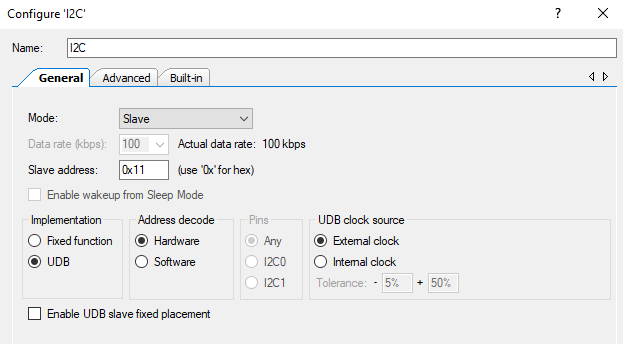
\includegraphics[width=0.75\textwidth]{Softwaredesign/RPI_IF/graphics/i2c_settings.PNG}
    \caption{Konfiguering af I2C slave enhed.}
    \label{fig:i2c_settings}
\end{figure}

\textbf{sendCupStatus}\\
En af klassens formål er at sende CupStatus beskeder til RPI'en, når en opdatering af variablen forekommer. Dette gøres  via en funktion i boundary klassen kaldet sendCupStatus. Denne funktion tager en parameter af typen uint8, som er en byte, der beskriver cup status. For mere information refereres igen til grænseflade afsnittet i software arkitekturen afsnit \fullref{arch:sec:RPi_Playerside_com}. Funktionen starter med at resette readbufferen fra i2c slave enheden(Vi skal selv lave bufferen, som gjort ved writebufferen) ved at lægge 0xFF ind på alle pladser i bufferen. Cup status bliver herefter lagt over i bufferen, så RPI'en kan læse det. Herefter bliver funktionen I2C\_SlaveClearReadBuf kaldt for at resette bufferen(pointer peger nu rigtigt til første plads i bufferen). Det sidste Der gøres er at interrupt benet skal trækkes lavt, så et interrupt skabes på RPI'en, hvorved der vil blive læst fra Read bufferen.  Efter dette skal interrupt benet trækkes højt igen efter et meget kort delay, da RPI driveren reagerer på en falling edge.

\textbf{RPI\_IF\_handledata}\\
Den anden og sidste funktion i denne klasse, der ikke bare er en hjælpefunktion(Der er også en initiations funktion for slave enheden) er RPI\_IF\_handledata. Denne funktion står for modtagelsen af beskeder fra RPI'en. Det første den gør er at tjekke for om slave enhedens "write complete" flag er sat i slaveenhedens status register. Hvis dette flag er sat, er det fordi en besked er sendt til PSoC'en. I et for loop vil der blive loop'et med det antal bytes, der er i bufferen, så alt sendt data vil blive læst. Inde i for loop'et er der et switch statement, der ser på den først byte sendt, hvis den svarer til enten en "state" ændring(0x0A til 0x0E) eller en farvekode(0x21), så vil den tilhørende case eksekveres. Ved "state" ændring vil setState blive kaldt og når en farve kode sendes er det enten setMyColor eller setOpponentColor, der bliver kaldt. De er alle funktioner i GameController klassen. Når en besked er læst, så vil I2C\_SlaveClearWriteBuf kaldes for en sikkerhedsskyld, selvom en ny besked sendt til PSoC'en også vil forårsage, at buffer pointeren bliver nulstillet(peger mod første element i bufferen). Man vil se at der i denne funktion er brugt et struct color\_t. Dette struct forklares, der mere om i CupLight\_IF design i afsnit \fullref{swdesign:sec:cuplight_sw_design}.
\end{document}